
The main strength of algorithm~\ref{algo:hybrid--dynamic-fp} lies in the fact that we can focus on the solutions pointwise without having to deal with global structures, thus somewhat mitigating the curse of dimensionality. Also, generating trajectories for the Feynman-Kac expectation with Euler-Maruyama lends itself to extreme parallelization, a must-have ingredient for solving high dimensional problems. The nature of the algorithm makes it applicable to a fairly large set of problems. Moreover, to compute solutions for the same problem but different initial conditions one can just reuse the same trajectory data and once the trajectory data are generated, solutions can be found for all of the time-points used to generate the trajectory data.

The limitations of algorithm~\ref{algo:hybrid--dynamic-fp} closely related to the properties dynamical system we are dealing with. In order to explore these, first, we need to explore the behavior of the h-SDE \eqref{eq:h-SDE--dynamic-fp} for different dynamical systems.
\subsubsection{Behavior of h-SDE trajectories and domain contraction}\label{ssec-h-behavior--dynamic-fp}
The stationary Fokker-Planck equation $\mathcal Lp_\infty=0$ has analytical solution for gradient systems. In this case, the solution can be expressed as 
\begin{align}
    &p_\infty\propto \exp\left(-\frac{2V}{\sigma^2}\right)\\
    \implies&\sigma^2\nabla\log p_{\infty} = 2\mu\\
    \implies&\bar{\mu}=\mu
\end{align}
where $V$ is defined as in \eqref{eq:grad-mu--dynamic-fp}, for a derivation see for example, section~3.1 in \cite{mandal2023learning}. Consequently, the h-SDE for gradient systems can be written as 
\begin{align}
    d\bar X_t = \mu\, dt+\sigma\, dW_t\label{eq:h-SDE-grad--dynamic-fp}
\end{align}
So for the gradient case, the h-SDE is identical to the original SDE \eqref{eq:SDE-0--dynamic-fp} describing the underlying dynamical system. Since the dynamical system possesses an attractor, the trajectories of the h-SDE are attracted to this this attractor and we can safely avoid blow-up even if the drift $\mu$ is non-Lipschitz.

But the same can not be said for the non-gradient systems where the where the drift term $\bar{\mu}$ in the h-SDE might be dominated by $-\mu$ rather than being $\mu$ as in the original SDE, thus losing its attracting properties. In such cases the solutions of the h-SDE might experience finite or infinite time blow-up.
\begin{figure}[!ht]
    \centering
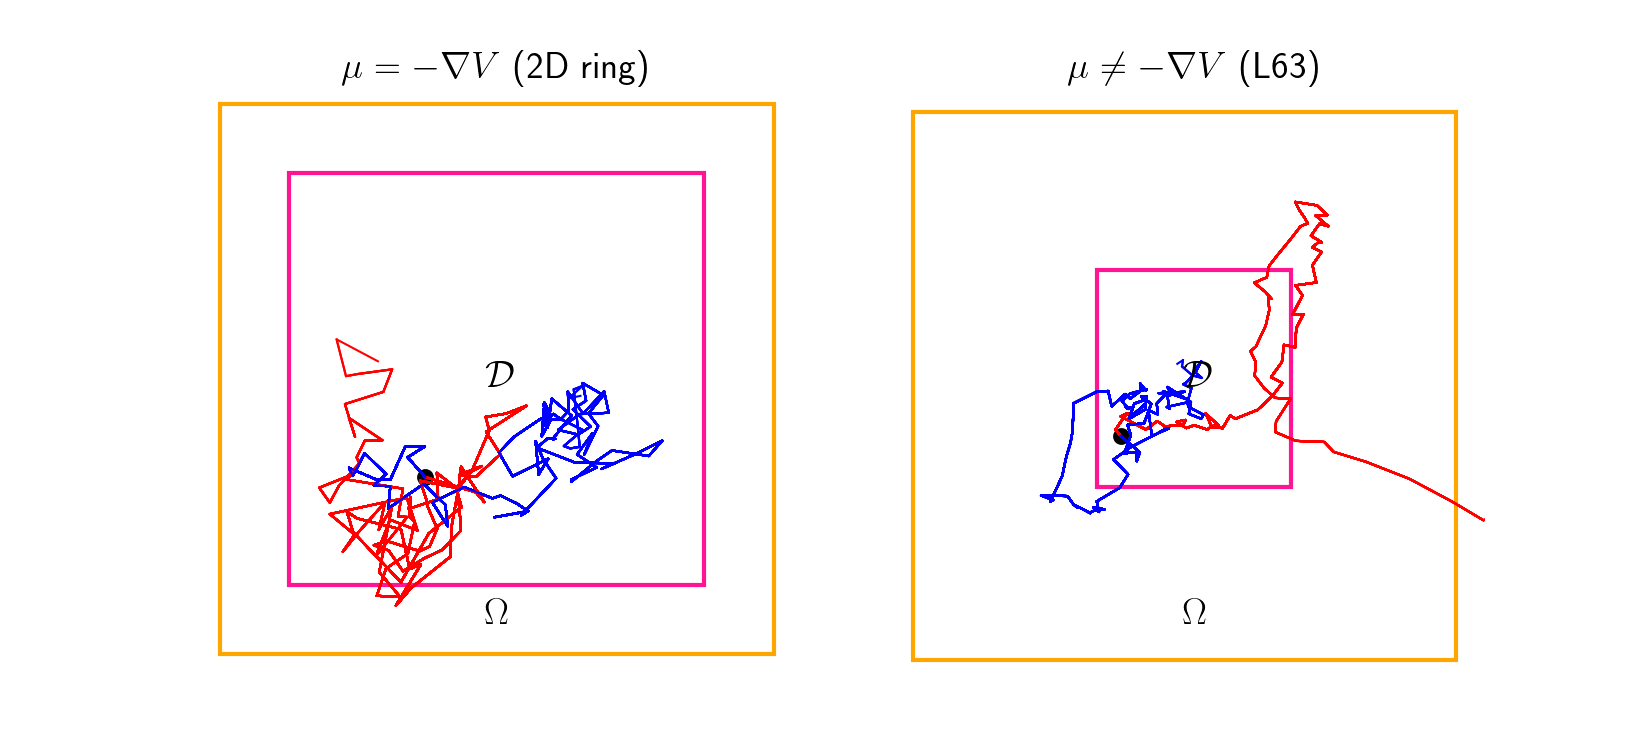
\includegraphics[scale=0.55]{dynamic-fp/plots/dynamic-plots-h-SDE.png}
    \caption{h-SDE trajectories for various systems. In both cases a pair of trajectories start from the same point (depicted as a black dot) in $\mathcal D$. While the trajectories for the gradient system might leave $\mathcal D$ (smaller rectangle), they do not leave $\Omega$ (larger rectangle). However, the same is not true for the non-gradient system.}
    \label{fig:h-SDE--dynamic-fp}
\end{figure}

Our knowledge of $\bar{\mu}$ is determined by our knowledge of $p_\infty$. If we do not have an analytic form for $p_\infty$ and have computed $p_\infty$ (up to the normalization constant) only up to the domain $\Omega$ then we can only be sure of our knowledge of $\bar{\mu}$ up to the domain $\Omega$. Consequently, if we want to compute the solution on the domain $\mathcal D$ then we must select $\mathcal D\subset\Omega$ in a way such that the trajectories of h-SDE that start inside $\mathcal D$, do not leave $\Omega$ till time $T$ with high probability. To quantify this notion, we can choose a tolerance $\varepsilon>0$ and select $\mathcal D, T$ such that,


\begin{align}
    \xi(T, \mathcal D, \Omega)\stackrel{\rm def}{=}\mathbb E_{\mathbf x\sim U(\mathcal D)}[P(\bar X_t\in\Omega\;\forall\;t\in[0, T]|\bar X_0=\mathbf x)] > 1-\varepsilon\label{eq:xi-defn--dynamic-fp}
\end{align}

$\xi(T, \mathcal D, \Omega)$ denotes the average probability that a trajectory stays inside $\Omega$ till time $T$ given that it started inside $\mathcal D$, $U(\mathcal D)$ denotes the uniform distribution on $\mathcal D$ in \eqref{eq:xi-defn--dynamic-fp}. $\xi$ helps us specify the space-time boundaries for the effective employment of algorithm~\ref{algo:hybrid--dynamic-fp}. While for a gradient system, choosing $\Omega$ such that it contains the corresponding attractor, we can make sure that h-SDE trajectories originating from $\mathcal D$ do not leave $\Omega$ with high probability, the same can not be said for a non-gradient system. Figure~\ref{fig:h-SDE--dynamic-fp} shows the difference between h-SDE trajectories for typical gradient and non-gradient systems. Since for gradient systems the h-SDE trajectories do not leave $\Omega$ with high probability, $\xi(T, \mathcal D, \Omega)\approx 1$ for any $T$. In fact, empirically it might evaluate exactly to $1$. But for non-gradient system $\xi(T, \mathcal D, \Omega)$ is a decreasing function of $T$ as seen in figure~\ref{fig:xi--dynamic-fp} and in such cases we select the hyperparameter $T$ for algorithm~\ref{algo:hybrid--dynamic-fp} according to \eqref{eq:xi-defn--dynamic-fp} using a pre-chosen tolerance $\varepsilon$.

\begin{figure}[!ht]
    \centering
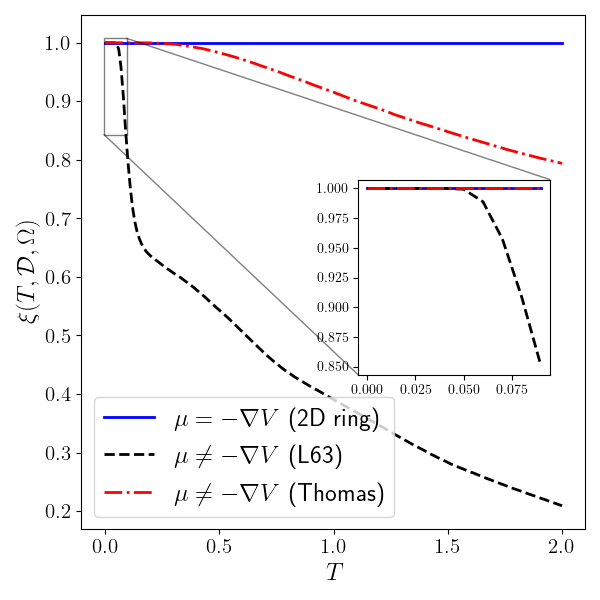
\includegraphics[scale=0.5]{dynamic-fp/plots/dynamic-plots-xi.png}
    \caption{$\xi(T, \mathcal D, \Omega)$ as a function of $T$ for various systems.}
    \label{fig:xi--dynamic-fp}
\end{figure}


We are only able to solve \eqref{eq:FPE-0--dynamic-fp} on a subset $\mathcal D$ of where we solved its stationary counterpart, namely $\Omega$. We refer to this phenomenon as \textit{domain contraction}. Even though we have included gradient systems in the figures~\ref{fig:h-SDE--dynamic-fp}, \ref{fig:xi--dynamic-fp} for expository purposes, since we have perfect knowledge of $p_\infty$ (up to the normalization constant) over entire $\mathbb R^d$, domain contraction is a practical issue only for non-gradient systems and $T$ can be chosen arbitrarily large for gradient systems. 


\subsubsection{Interpretation of finite time viability for non-gradient systems via Feynman-Kac on finite domains}\label{ssec-interpret-FK-finite--dynamic-fp}
Since we are dealing with finite domains, we can also look at the h-SDE through the lens of the Feynman-Kac formula on finite domains. In order to apply the finite domain version of the Feynman-Kac formula one requires perfect knowledge of the solution at the boundary at all times. In our case we need to know $h(t, \mathbf x)$ on $([0, T)\times{\partial\Omega}) \cup (\{0\}\times\bar{\Omega})$. For the ease of discussion let us define the following quantity,
\begin{align}
    h(t, \mathbf x) = \begin{cases}
        &\Psi(T, \mathbf x),\;\forall\;\mathbf x\in \bar{\Omega},\; t=0\\
        & \Psi(T-t, \mathbf x)\;\forall\;(t,\mathbf x)\in[0, T)\times\partial\Omega
    \end{cases}
\end{align}
Assuming we know $\Psi$, the Feynman-Kac formula for $h$ becomes,
\begin{align}
    h(t, \mathbf x) = \mathbb E\left[\left.\Psi(\tau\wedge T, \bar{X}_{\tau\wedge T})\right\vert \bar X_0=\mathbf x\right]\label{eq:h-E-finite--dynamic-fp}
\end{align}
where $\tau$ denotes the first exit-time of $\bar{X}$ for $\Omega$ or,
\begin{align}
    \tau(\mathbf x) \stackrel{\rm def}{=} \inf\{s>0: \bar X_s\not\in\Omega\} 
\end{align}
For derivations of such formulae the interested reader can refer to theorem~4.4.5 in \cite{gobet2016monte} or theorem~4.2 in chapter~7 of \cite{yong1999stochastic} and its preceding section. Since in reality we only know $h(t, \mathbf x)$ at $t=0$ and therefore have no knowledge of $\Psi(T-t, \mathbf x)$ at any point other than $t=0$, we can hope to effectively use \eqref{eq:h-E-finite--dynamic-fp} only if the trajectories of h-SDE do not exit $\Omega$ till time $T$ with high probability. In such a scenario $\tau\wedge T$ becomes equal to $T$ and we are not forced to evaluate $\Psi$ at any point where we have no knowledge of $\Psi$. Using the finite domain version of Feynman-Kac therefore leads us to similar conclusions as in the previous section, namely, algorithm~\ref{algo:hybrid--dynamic-fp} can be used to solve gradient and non-gradient systems up to arbitrarily large and finite times respectively.

\subsubsection{Effect allowing h-SDE trajectories to leave \texorpdfstring{$\Omega$}{Lg} in case of perfect knowledge of \texorpdfstring{$p_\infty$ in $\Omega$}{Lg}}\label{sssec-error--dynamic-fp}
 Since $p_\infty$ is not computed by algorithm~\ref{algo:hybrid--dynamic-fp} but rather is an input to it, a scenario of interest is when we have perfect (rather than approximate) knowledge of $p_\infty$ on $\Omega$. In such a scenario we would like the algorithm to produce reasonably good approximate solutions even when we are willing tolerate $\xi(T, \mathcal D, \Omega)\neq1$ or some h-SDE trajectories leaving $\Omega$ within our chosen $T$. To analyze this scenario let us define our knowledge of $p_\infty$ as,
 \begin{align}
     \hat p_\infty(\mathbf x) =\begin{cases}
         &p_\infty(\mathbf x), \qquad\mathbf x\in\Omega\\
         &p_\infty^\sharp(\mathbf x),\qquad\mathbf x\in\Omega^c
     \end{cases} 
 \end{align}
 where $p_\infty^\sharp\neq p_\infty$ represents imperfect knowledge of $p_\infty$ outside $\Omega$. Similarly we can define a modified h-SDE as,
 \begin{align}
     d\hat X_t = (\sigma^2\nabla\log \hat p_\infty -\mu)\,dt+\sigma\,dW_t
 \end{align} 
 and the corresponding solution generated by algorithm~\ref{algo:hybrid--dynamic-fp} as,
 \begin{align}
   &\hat h(t, \mathbf x) = \mathbb E\left[\left.\frac{p_0(\hat{X}_t)}{\hat{p}_\infty(\hat{X}_t)}\right\vert \hat{X}_0=\mathbf x\right]\\
   & \hat p(t ,\mathbf x)=\hat h(t, \mathbf x) \hat p_\infty(\mathbf x)
\end{align}
Now we are ready to analyze the pointwise error incurred when we allow h-SDE trajectories to escape $\Omega$ within time $T$ with probability less than $\varepsilon$ or $\xi(T, \mathcal D, \Omega)>1-\varepsilon$.
\begin{prop}Let $\bar E, \hat E$ be the events\footnote{Note that $\bar E, \hat E$ are events dependent on $t, \mathbf x$ but to avoid notational cluttering we do not make this dependence explicit.} that $\bar X, \hat X$ stay inside $\Omega$ till time $t$ after starting at $\mathbf x\in\mathcal D\subset\Omega$ respectively. Assume the following,
    \begin{enumerate}
    \item $\xi(T, \mathcal D, \Omega)>1-\varepsilon$
    % \item  \begin{align}\mathbb E_{\mathbf x\sim U(\mathcal D)}[P(\hat E)]\le1-\varepsilon>0\;\forall\;t\in[0, T]\end{align}
    
    \item $\exists$ a constant $K>0$ such that,
    \begin{align} 
     p_\infty(\mathbf x)\,\mathbb E[ h_0(\bar X_t)|\bar X_0=\mathbf x, \bar E^c],\;\hat p_\infty(\mathbf x)\,\mathbb E[\hat h_0(\hat X_t)|\hat X_0=\mathbf x, \hat E^c] < K \;\forall\;\mathbf (t,\mathbf x)\in[0, T]\times\mathcal D
    \end{align}
    where,\begin{align}
    &h_0 \stackrel{\rm def}{=} \frac{p_0}{p_\infty}\\
    &\hat h_0 \stackrel{\rm def}{=} \frac{p_0}{\hat p_\infty}
\end{align}
\end{enumerate}
Then, 
\begin{align}
    \mathbb E_{\mathbf x\sim U(\mathcal D)}[|\hat p(t, \mathbf x)-p(t, \mathbf x)|] \le 2K\varepsilon\;\forall\;t\in[0, T]
    \label{eq:pt-error--dynamic-fp}
\end{align}\label{prop:escape--dynamic-fp}
\end{prop}
\begin{proof}
Let $\mathbf x\in\mathcal D$ and $\Delta_h = h_0-\hat h_0$.
    \begin{align}
    |\hat p(t, \mathbf x)-p(t, \mathbf x)| = |\Delta_1+\Delta_2|    
    \end{align}
where
\begin{align}
    \Delta_1 =  p_\infty(\mathbf x)\,\mathbb E\left[\left.\frac{p_0(\bar{X}_t)}{{p}_\infty(\bar{X}_t)}\right\vert \bar{X}_0=\mathbf x\right]-\hat p_\infty(\mathbf x)\,\mathbb E\left[\left.\frac{p_0(\bar{X}_t)}{\hat{p}_\infty(\bar{X}_t)}\right\vert \bar{X}_0=\mathbf x\right]
\end{align}
and,
\begin{align}
    \Delta_2 = \hat p_\infty(\mathbf x)\,\mathbb E\left[\left.\frac{p_0(\bar{X}_t)}{\hat{p}_\infty(\bar{X}_t)}\right\vert \bar{X}_0=\mathbf x\right]-\hat p_\infty(\mathbf x)\,\mathbb E\left[\left.\frac{p_0(\hat{X}_t)}{\hat{p}_\infty(\hat{X}_t)}\right\vert \hat{X}_0=\mathbf x\right]
\end{align}
Now note that, 
\begin{align}
    \Delta_1 = &p_\infty(\mathbf x)\,\mathbb E[h_0(\bar X_t)|\bar X_0=\mathbf x, \bar E]\,P(\bar E)+p_\infty(\mathbf x)\,\mathbb E[h_0(\bar X_t)|\bar X_0=\mathbf x, \bar E^c]\,(1-P(\bar E))\\
    -&\hat p_\infty(\mathbf x)\,\mathbb E[\hat h_0(\bar X_t)|\bar X_0=\mathbf x, \bar E]\,P(\bar E)-\hat p_\infty(\mathbf x)\,\mathbb E[\hat h_0(\bar X_t)|\bar X_0=\mathbf x, \bar E^c]\,(1-P(\bar E))
\end{align}
Recalling that we have perfect knowledge of $p_\infty$ inside $\Omega$ we get,
\begin{align}
    \Delta_1=&p_\infty(\mathbf x)\left[\mathbb E[\Delta_h(\bar X_t)|\bar X_0=\mathbf x, \bar E]\,P(\bar E)+\mathbb E[\Delta_h(\bar X_t)|\bar X_0=\mathbf x, \bar E^c]\,(1-P(\bar E))\right]\\
    =&p_\infty(\mathbf x)\,\mathbb E[\Delta_h(\bar X_t)|\bar X_0=\mathbf x, \bar E^c]\,(1-P(\bar E))
\end{align}
where we arrive at the last equality by noticing that $\Delta_h=0$ in the event of $\bar E$.
And,
\begin{align}
    \Delta_2 = &\hat p_\infty(\mathbf x)\,[\mathbb E[\hat h_0(\bar X_t)|\bar X_0=\mathbf x, \bar E]\,P(\bar E)+\mathbb E[\hat h_0(\bar X_t)|\bar X_0=\mathbf x, \bar E^c]\,(1-P(\bar E))]\\
    -&\hat p_\infty(\mathbf x)\,[\mathbb E[\hat h_0(\hat X_t)|\hat X_0=\mathbf x, \hat E]\,P(\hat E)+\mathbb E[\hat h_0(\hat X_t)|\hat X_0=\mathbf x, \hat E^c]\,(1-P(\hat E))]
\end{align}
  Since $\bar X, \hat X$ follow identical dynamics inside $\Omega$, $P(\bar E)=P(\hat E)$ and we have,
\begin{align}
    \Delta_2 = &\hat p_\infty(\mathbf x)\,[\mathbb E[\hat h_0(\bar X_t)|\bar X_0=\mathbf x, \bar E^c]-\mathbb E[\hat h_0(\hat X_t)|\hat X_0=\mathbf x, \hat E^c]]\,(1-P(\hat E))
\end{align}
\end{proof}
Again noting $\hat p_\infty(\mathbf x)=p_\infty(\mathbf x)$ and $P(\bar E)=P(\hat E)$ we get,
\begin{align}
    \Delta_1+\Delta_2 = & [p_\infty(\mathbf x)\,\mathbb E[ h_0(\bar X_t)|\bar X_0=\mathbf x, \bar E^c]-\hat p_\infty(\mathbf x)\,\mathbb E[\hat h_0(\hat X_t)|\hat X_0=\mathbf x, \hat E^c]]\,(1-P(\hat E))\\
    \implies|\Delta_1+\Delta_2|\le&2K\,(1-P(\hat E))
\end{align}
Since $\xi$ is a monotone decreasing function of its first argument, the first assumption is equivalent to,
\begin{align}
    \xi(t, \mathcal D, \Omega) > 1-\varepsilon\;\forall\; t\in[0, T]
\end{align}
Therefore, according to the definition of $\xi$,
\begin{align}
    \mathbb E_{\mathbf x\sim U(\mathcal D)}[P(\bar E)] > 1-\varepsilon \;\forall\;t\in[0, T]
\end{align}
which implies,
\begin{align}
    &\mathbb E_{\mathbf x\sim U(\mathcal D)}[1-P(\hat E)] <\varepsilon \;\forall\;t\in[0, T]\\
    \implies&\mathbb E_{\mathbf x\sim U(\mathcal D)}[|\Delta_1+\Delta_2|]<2K\varepsilon
\end{align}
which completes our proof.

The second assumption in proposition~\ref{prop:escape--dynamic-fp} makes sure if we compute the probability densities using only the trajectories that exit $\Omega$ before time $t$, we get bounded quantities independent of $\varepsilon$. Proposition~\ref{prop:escape--dynamic-fp} tells us\textit{, under suitable circumstances, the average error that is caused by allowing some h-SDE trajectories to leave $\Omega$ is proportional to the fraction of trajectories that leave $\Omega$.} If we modify the first assumption to require that the inequality holds pointwise for every $\mathbf x\in\mathcal D$ instead, we can bound the supremum norm of the error over $\mathcal D$ instead of the average error.